\documentclass[11pt,a4paper]{article}
\usepackage[T1]{fontenc}
\usepackage[utf8]{inputenc}
\usepackage{lmodern}
\usepackage[margin=2.3cm]{geometry}
\usepackage{graphicx}
\graphicspath{{../img/}}
\usepackage{xcolor}
\definecolor{spblue}{HTML}{1F4E79}
\definecolor{spteal}{HTML}{2C7A7B}
\usepackage{booktabs}
\usepackage{longtable}
\usepackage{array}
\usepackage{enumitem}
\usepackage{float}
\usepackage{caption}
\captionsetup{font=small,labelfont=bf}
\usepackage{listings}
\lstset{basicstyle=\ttfamily\footnotesize,breaklines=true,frame=single,backgroundcolor=\color{gray!8},columns=fullflexible,keepspaces=true}
\usepackage[hidelinks]{hyperref}
\usepackage{titlesec}
\titleformat{\section}{\color{spblue}\Large\bfseries}{\thesection}{0.6em}{}
\titleformat{\subsection}{\color{spteal}\large\bfseries}{\thesubsection}{0.6em}{}
\setlength{\parskip}{0.5em}\setlength{\parindent}{0pt}

\title{ScholarPath --- The Conceptual ERD (Step 1)\\[0.3em]
\large A Four-Part Data-Modelling Series: Part 1 of 4}
\author{ScholarPath Team}
\date{}

\begin{document}
\maketitle

\begin{abstract}
\noindent
This is the first instalment of a four-part teaching series that walks the
ScholarPath data model through the classic database-design pipeline:
\textbf{plain ERD $\rightarrow$ Enhanced ER (EERD) $\rightarrow$ Relational
Mapping $\rightarrow$ Class Diagrams}. The present document establishes the
\emph{conceptual} starting point --- a deliberately plain Entity--Relationship
Diagram (ERD) drawn in Chen / Elmasri notation. We introduce the ScholarPath
platform and its four actors, recall the vocabulary of the ER model (entities,
relationships, attributes, keys and the $1$/$N$/$M$ cardinality ratios), and
then present the basic conceptual diagram of roughly fifteen core entities and
their relationships. Crucially, this is the ``before'' picture: at this stage
the model is intentionally flat --- a single \texttt{USER} entity with role as a
mere attribute, no specialization, no weak entities, and no multivalued or
derived attributes. Those simplifications are exactly what \emph{Part~2: The
Enhanced ER Diagram} sets out to repair, so this document closes by motivating
that enhancement.
\end{abstract}

\tableofcontents

\section{Introduction to the ScholarPath System}

\textbf{ScholarPath} is a web platform that connects students seeking
educational funding with the people and organisations that can help them obtain
it. In a single application it brings together a scholarship catalogue and
application tracker, a paid consultant-booking and session-recording service, a
paid company review service for applications, a community forum with private
chat, a resources hub, and a layer of analytics and AI-assisted recommendation.
The system is built as a .NET backend with a React front end; this series,
however, is concerned only with the \emph{data model} that underpins it.

\subsection{The four actors}

Every interaction in ScholarPath is performed by one of four kinds of user. In
the running system these are roles granted to a single account principal, but
conceptually they behave as four distinct actors:

\begin{itemize}[leftmargin=1.4em]
  \item \textbf{Student} --- the primary beneficiary. A student maintains an
        academic profile (academic level, field of study, GPA, preferred
        countries), discovers and applies to scholarships, uploads supporting
        documents, books paid consultant sessions, requests paid company
        reviews of an application, and participates in the community.
  \item \textbf{Company} --- an organisation that owns and publishes
        scholarships, and that can be paid to review a student's application.
        A company carries an organisation legal name, a verification status and
        an aggregate rating.
  \item \textbf{Consultant} --- a domain expert who publishes availability,
        conducts paid one-to-one booking sessions, and is rated afterwards. A
        consultant carries a session fee, expertise tags and a payout
        (Stripe Connect) status.
  \item \textbf{Admin} --- the platform operator who moderates content,
        approves verification and upgrade requests, and configures the
        platform.
\end{itemize}

\subsection{Main subject areas}

The platform's data naturally clusters into six subject areas, all radiating
from the user. These same clusters reappear, in much greater detail, in the
later parts of this series:

\begin{enumerate}[leftmargin=1.6em]
  \item \textbf{Identity \& Profile} --- accounts, roles and profile data.
  \item \textbf{Scholarships, Applications \& Documents} --- the catalogue, the
        applications students submit against it, the documents that support
        them, and paid company reviews.
  \item \textbf{Booking, Payments \& Ratings} --- consultant availability,
        bookings, the payments that settle them, and the reviews that follow.
  \item \textbf{Community \& Chat} --- forum posts and private conversations.
  \item \textbf{Resources \& Notifications} --- learning resources and the
        notifications that keep users informed.
  \item \textbf{AI, Knowledge \& Platform} --- recommendation, the knowledge
        base, auditing and configuration.
\end{enumerate}

This first document zooms out to the most important entities across these areas
and draws them plainly. The companion document \emph{Part~2: The Enhanced ER
Diagram} adds the structural refinements; \emph{Part~3: Relational Mapping}
turns the model into tables; and \emph{Part~4: Class Diagrams} expresses it in
object-oriented terms.

\section{What an ERD Is}

The \textbf{Entity--Relationship Diagram (ERD)} is the standard conceptual tool
for describing the structure of data independently of any particular database
technology. It was introduced by Peter Chen and is presented here in the
\textbf{Chen / Elmasri} notation used throughout most database textbooks. The
notation rests on four building blocks.

\subsection{Entities and entity types}

An \textbf{entity} is a real-world object or concept about which we store data
--- a particular scholarship, a particular booking, a particular user. An
\textbf{entity type} is the named category to which such objects belong (for
example \texttt{SCHOLARSHIP}). In Chen notation an entity type is drawn as a
\textbf{rectangle}.

\subsection{Attributes}

An \textbf{attribute} is a property of an entity type --- a scholarship has a
title, a deadline and a status. Attributes are drawn as \textbf{ovals}
connected to their entity rectangle. The conceptual model deliberately records
only the few attributes that matter for understanding the structure, not the
full column list (that is the job of Part~3).

\subsection{Keys}

A \textbf{key} attribute uniquely identifies each entity of a type --- no two
entities may share the same key value. In Chen notation a key attribute is
\textbf{underlined}. In ScholarPath every core entity is keyed by an
\texttt{Id}, shown underlined in the diagram.

\subsection{Relationships}

A \textbf{relationship} is a meaningful association between entities --- a user
\emph{submits} an application; a booking is \emph{settled by} a payment.
A \textbf{relationship type} is drawn as a \textbf{diamond} on the line that
joins the participating entity rectangles, labelled with a verb.

\subsection{Cardinality ratios: 1, N and M}

The \textbf{cardinality ratio} of a binary relationship records how many
entities of one type may be associated with the other. Each end of the
relationship line is marked with a symbol:

\begin{itemize}[leftmargin=1.4em]
  \item \textbf{1} --- ``one''. At most one entity participates on this side.
  \item \textbf{N} (or \textbf{M}) --- ``many''. Any number of entities may
        participate on this side.
\end{itemize}

This yields the three classic shapes summarised in Table~\ref{tab:cardinality}.

\begin{table}[H]\centering
\caption{The three cardinality ratios in Chen notation.}
\label{tab:cardinality}
\begin{tabular}{@{}lll@{}}
\toprule
\textbf{Ratio} & \textbf{Reads as} & \textbf{ScholarPath example} \\
\midrule
1\,:\,1 (one-to-one)   & one $A$ relates to one $B$        & a booking is rated by at most one consultant review \\
1\,:\,N (one-to-many)  & one $A$ relates to many $B$       & one user submits many applications \\
M\,:\,N (many-to-many) & many $A$ relate to many $B$       & a user participates in many conversations, each with many users \\
\bottomrule
\end{tabular}
\end{table}

\section{The Basic Conceptual ERD}

Figure~\ref{fig:erd-basic} presents the basic conceptual ERD for ScholarPath in
authentic Chen notation: rectangles are entity types, diamonds are relationship
types, ovals are attributes, underlined attributes are keys, and the
\texttt{1}/\texttt{N}/\texttt{M} markers on the edges give the cardinality
ratios. It is the source diagram for everything that follows in this series.

\begin{figure}[H]\centering
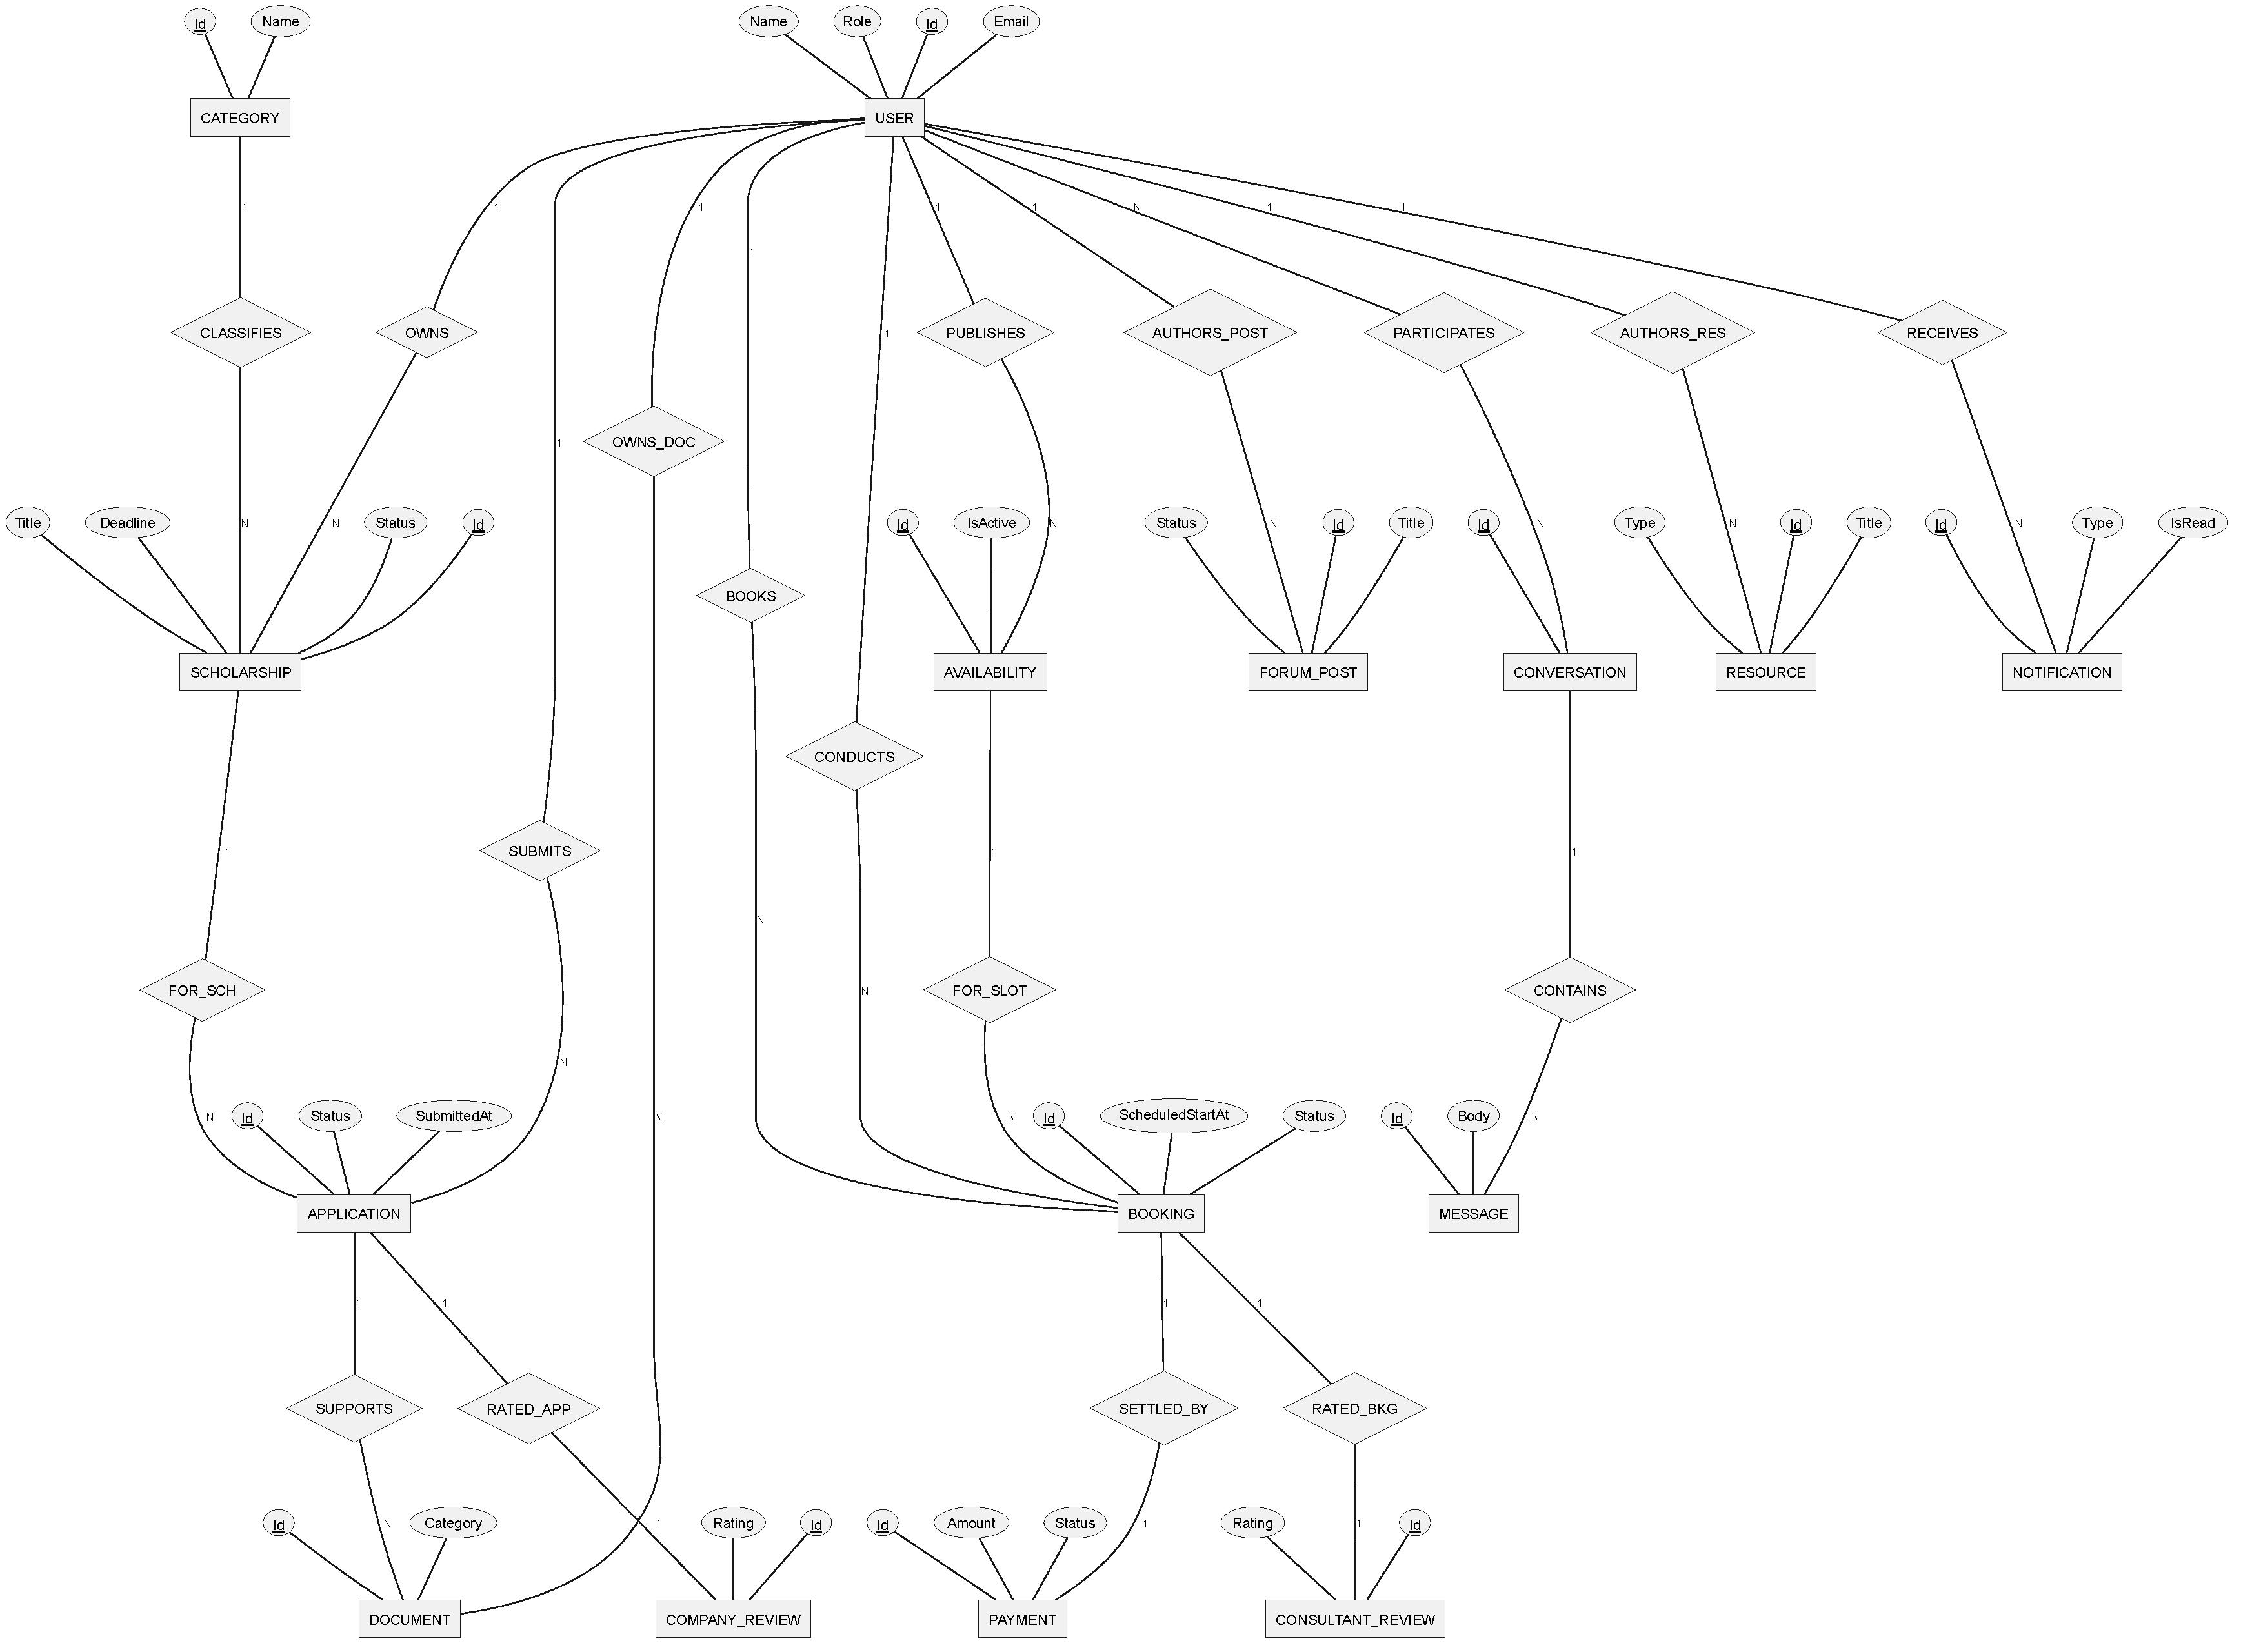
\includegraphics[width=\linewidth,height=0.82\textheight,keepaspectratio]{ScholarPath_ERD_Basic.pdf}
\caption{The basic conceptual ERD for ScholarPath in Chen / Elmasri notation
--- the deliberately plain starting point. \texttt{USER} is a single flat
entity whose \texttt{Role} is just an attribute.}
\label{fig:erd-basic}
\end{figure}

\subsection{The core entities}

The diagram captures fifteen core entity types. Table~\ref{tab:entities} lists
each one with its meaning and the key attributes shown on the conceptual
diagram.

\begin{longtable}{@{}>{\raggedright\arraybackslash}p{2.9cm}>{\raggedright\arraybackslash}p{8.5cm}>{\raggedright\arraybackslash}p{2.6cm}@{}}
\caption{The fifteen core entity types of the basic ScholarPath ERD.}
\label{tab:entities}\\
\toprule
\textbf{Entity} & \textbf{Meaning} & \textbf{Key / shown attributes} \\
\midrule
\endfirsthead
\toprule
\textbf{Entity} & \textbf{Meaning} & \textbf{Key / shown attributes} \\
\midrule
\endhead
\bottomrule
\endfoot
\texttt{USER} & Any account holder. At this stage \texttt{Role} is just an attribute distinguishing Student, Company, Consultant and Admin. & \underline{Id}, Email, Name, Role \\
\texttt{CATEGORY} & A subject classification applied to scholarships. & \underline{Id}, Name \\
\texttt{SCHOLARSHIP} & A funding opportunity that students apply to. & \underline{Id}, Title, Deadline, Status \\
\texttt{APPLICATION} & A student's submission against a scholarship. & \underline{Id}, Status, SubmittedAt \\
\texttt{DOCUMENT} & A file uploaded to support an application. & \underline{Id}, Category \\
\texttt{COMPANY\_REVIEW} & A company's rating of a reviewed application. & \underline{Id}, Rating \\
\texttt{AVAILABILITY} & A time slot a consultant publishes for booking. & \underline{Id}, IsActive \\
\texttt{BOOKING} & A booked consultant session. & \underline{Id}, ScheduledStartAt, Status \\
\texttt{PAYMENT} & A money settlement for a booking. & \underline{Id}, Amount, Status \\
\texttt{CONSULTANT\_REVIEW} & A student's rating of a completed booking. & \underline{Id}, Rating \\
\texttt{FORUM\_POST} & A post in the community forum. & \underline{Id}, Title, Status \\
\texttt{CONVERSATION} & A private chat channel between users. & \underline{Id} \\
\texttt{MESSAGE} & A single message inside a conversation. & \underline{Id}, Body \\
\texttt{RESOURCE} & A learning resource authored on the platform. & \underline{Id}, Title, Type \\
\texttt{NOTIFICATION} & A message delivered to a user. & \underline{Id}, Type, IsRead \\
\end{longtable}

\subsection{The relationships and their cardinalities}

Table~\ref{tab:relationships} walks through every relationship drawn in
Figure~\ref{fig:erd-basic}, in the order it appears in the diagram, giving the
participating entities, the relationship verb and the cardinality ratio. All
but one relationship are one-to-many; the lone many-to-many is the
\textsc{participates} link between users and conversations.

\begin{longtable}{@{}>{\raggedright\arraybackslash}p{3.0cm}>{\raggedright\arraybackslash}p{2.4cm}>{\raggedright\arraybackslash}p{3.0cm}cl@{}}
\caption{Relationships of the basic ScholarPath ERD with cardinality ratios.}
\label{tab:relationships}\\
\toprule
\textbf{From} & \textbf{Relationship} & \textbf{To} & \textbf{Ratio} & \textbf{Reads as} \\
\midrule
\endfirsthead
\toprule
\textbf{From} & \textbf{Relationship} & \textbf{To} & \textbf{Ratio} & \textbf{Reads as} \\
\midrule
\endhead
\bottomrule
\endfoot
USER          & \textsc{owns}          & SCHOLARSHIP       & 1\,:\,N & a company owns many scholarships \\
CATEGORY      & \textsc{classifies}    & SCHOLARSHIP       & 1\,:\,N & a category classifies many scholarships \\
USER          & \textsc{submits}       & APPLICATION       & 1\,:\,N & a student submits many applications \\
SCHOLARSHIP   & \textsc{for\_sch}      & APPLICATION       & 1\,:\,N & a scholarship receives many applications \\
APPLICATION   & \textsc{supports}      & DOCUMENT          & 1\,:\,N & an application is supported by many documents \\
USER          & \textsc{owns\_doc}     & DOCUMENT          & 1\,:\,N & a user owns many documents \\
APPLICATION   & \textsc{rated\_app}    & COMPANY\_REVIEW   & 1\,:\,1 & an application is rated by one company review \\
USER          & \textsc{publishes}     & AVAILABILITY      & 1\,:\,N & a consultant publishes many availability slots \\
USER          & \textsc{books}         & BOOKING           & 1\,:\,N & a student makes many bookings \\
USER          & \textsc{conducts}      & BOOKING           & 1\,:\,N & a consultant conducts many bookings \\
AVAILABILITY  & \textsc{for\_slot}     & BOOKING           & 1\,:\,N & a slot reserves many bookings \\
BOOKING       & \textsc{settled\_by}   & PAYMENT           & 1\,:\,1 & a booking is settled by one payment \\
BOOKING       & \textsc{rated\_bkg}    & CONSULTANT\_REVIEW& 1\,:\,1 & a booking is rated by one consultant review \\
USER          & \textsc{authors\_post} & FORUM\_POST       & 1\,:\,N & a user authors many forum posts \\
USER          & \textsc{participates}  & CONVERSATION      & M\,:\,N & users participate in many conversations \\
CONVERSATION  & \textsc{contains}      & MESSAGE           & 1\,:\,N & a conversation contains many messages \\
USER          & \textsc{authors\_res}  & RESOURCE          & 1\,:\,N & a user authors many resources \\
USER          & \textsc{receives}      & NOTIFICATION      & 1\,:\,N & a user receives many notifications \\
\end{longtable}

A few observations are worth making explicit, because they shape the story of
the later parts:

\begin{itemize}[leftmargin=1.4em]
  \item \textbf{\texttt{USER} is the hub.} Almost every relationship has
        \texttt{USER} on one side. The same account plays the part of company
        owner (\textsc{owns}), student applicant (\textsc{submits}),
        consultant (\textsc{publishes}, \textsc{conducts}) and student booker
        (\textsc{books}). The diagram cannot tell these roles apart --- they
        are all just ``\texttt{USER}''.
  \item \textbf{Two distinct roles on the same relationship target.} Both
        \textsc{books} and \textsc{conducts} connect \texttt{USER} to
        \texttt{BOOKING}; conceptually one end is a student and the other a
        consultant, but at this stage both are the same flat entity.
  \item \textbf{One-to-one review links.} \textsc{rated\_app},
        \textsc{settled\_by} and \textsc{rated\_bkg} are all $1{:}1$, capturing
        that an application has at most one company review, a booking has at
        most one payment, and a booking has at most one consultant review.
\end{itemize}

\section{Subject-Area Context}

Before drilling into structure, it helps to see how the entities group into the
six subject areas introduced in Section~1. Figure~\ref{fig:context} gives that
big-picture view, with \texttt{USER} at the centre and each subject area
hanging off it.

\begin{figure}[H]\centering

\includegraphics[width=\linewidth,height=0.82\textheight,keepaspectratio]{ScholarPath_Context.pdf}
\caption{Subject-area context. Everything radiates from \texttt{USER}; each
cluster is detailed in the later parts of this series.}
\label{fig:context}
\end{figure}

This context view is intentionally coarse: it shows \emph{which} groups of
entities exist and that they all touch the user, without committing to the
exact relationships. It is the map that the basic ERD of
Figure~\ref{fig:erd-basic} begins to fill in, and that Part~2 completes.

\section{Limitations of the Plain ERD}

The diagram in Figure~\ref{fig:erd-basic} is deliberately the ``before''
picture. It is a faithful, readable first cut, but it leaves several real
properties of the ScholarPath domain unexpressed. Naming these limitations is
not a criticism of the model --- it is precisely the agenda for
\emph{Part~2: The Enhanced ER Diagram}.

\subsection{USER is one flat entity --- role is just an attribute}

The most important simplification is that there is a single \texttt{USER}
entity, and the distinction between Student, Company, Consultant and Admin is
captured only by the \texttt{Role} attribute. This has visible consequences in
the diagram:

\begin{itemize}[leftmargin=1.4em]
  \item The role-specific attributes cannot be modelled. A student's academic
        level and GPA, a company's organisation legal name and verification
        status, and a consultant's session fee and expertise all belong to
        \emph{some} users but not others. A flat \texttt{USER} entity has no
        place to put them.
  \item The semantics of relationships are blurred. ``A \texttt{USER}
        \textsc{owns} a \texttt{SCHOLARSHIP}'' really means \emph{a company}
        owns it; ``a \texttt{USER} \textsc{books} a \texttt{BOOKING}'' really
        means \emph{a student} books it. The diagram cannot enforce or even
        state these role constraints.
\end{itemize}

\subsection{No specialization (no ISA hierarchy)}

Because \texttt{USER} is flat, there is \textbf{no specialization /
generalization}. The natural model is that \texttt{USER} is a super-type
specialized into Student, Company, Consultant and Admin sub-types, with the
sub-type-specific attributes attached to each sub-type. The plain ERD has no
way to draw the EER specialization circle or its disjoint/overlapping and
total/partial constraints. Adding this ISA hierarchy is the headline
enhancement of Part~2.

\subsection{No weak entities}

Every entity here is drawn as a strong (independent) entity with its own
\texttt{Id} key. The model does not express that some entities exist only as
\emph{parts} of a parent --- for example the per-chapter history of an
application or the children of a scholarship. Such existence-dependent
entities are properly modelled as \textbf{weak entities} (double rectangles,
identified through their owner), a refinement introduced in Part~2.

\subsection{No multivalued or derived attributes}

All attributes here are simple single-valued ones. The domain, however,
contains:

\begin{itemize}[leftmargin=1.4em]
  \item \textbf{Multivalued attributes} --- a consultant's expertise tags or a
        student's preferred countries are naturally a \emph{set} of values, not
        a single value. Chen notation draws these as double ovals; the plain
        ERD omits them entirely.
  \item \textbf{Derived attributes} --- a company's average rating or a
        scholarship's application count are \emph{computed} from related
        entities rather than stored independently. Chen notation draws these as
        dashed ovals; again, the plain ERD does not distinguish them.
\end{itemize}

\subsection{No distinction between enforced and loose references}

Finally, the plain ERD treats every relationship as equivalent. In the real
ScholarPath schema some associations are enforced by database foreign-key
constraints while others are deliberately ``loose'' application-level
references (used for high-volume audit, log and analytics data so that deleting
a user never cascade-breaks history). That distinction is a modelling decision
worth showing, and it too is introduced in the enhanced model.

\subsection{Why this matters --- the bridge to Part 2}

Taken together, these limitations are the motivation for the next document. The
plain ERD answers \emph{``what are the things and how are they broadly
related?''} The Enhanced ER Diagram answers the sharper questions the plain
model cannot: \emph{which} kind of user plays each role, which attributes are
multivalued or derived, which entities are existence-dependent, and which
references the database actually enforces.

\emph{Part~2: The Enhanced ER Diagram} takes the fifteen entities of
Figure~\ref{fig:erd-basic} and enriches them: it specializes \texttt{USER} into
its four sub-types, promotes the existence-dependent entities to weak entities,
adds the multivalued and derived attributes, and annotates the enforced-versus-
loose references. From there, \emph{Part~3: Relational Mapping} turns the
enhanced model into concrete tables, and \emph{Part~4: Class Diagrams} expresses
the same structure in object-oriented form. This document has set the stage by
drawing the honest, deliberately plain starting point.

\end{document}
